% \documentclass[german,master,buw]{webisthesis} % Weimar
\documentclass[english,bachelor,fsu]{webisthesis} % Jena
% \documentclass[german,bachelor,ul]{webisthesis} % Leipzig
% \documentclass[german,master,buw,web]{webisthesis} % Weimar, for web page
% \documentclass[german,bachelor,fsu,web]{webisthesis} % Jena, for web page
% \documentclass[german,bachelor,ul,web]{webisthesis} % Leipzig, for web page
%
% Non-default programme
% ---------------------
% \documentclass[english,master,buw]{webisthesis}\global\thesisprogramme{Human-Computer Interaction}
% \documentclass[english,master,buw]{webisthesis}\global\thesisfrontpagefaculty{Faculty of Civil Engineering/Faculty of Media}\global\thesisprogramme{Digital Engineering}
% \documentclass[german,bachelor,buw]{webisthesis}\global\thesisprogramme{Informatik\\Schwerpunkt Medieninformatik}
% \documentclass[german,bachelor,buw]{webisthesis}\global\thesisprogramme{Informatik\\Schwerpunkt Security and Data Science}
%
% When you change the language, pdflatex may halt on recompilation.
% Just hit enter to continue and recompile again. This should fix it.


%
% Values
% ------
\ThesisSetTitle{Analyzing Toxicity on Mastodon}
\ThesisSetKeywords{These, are, my, Keywords} % only for PDF meta attributes
\ThesisSetLocation{Jena} 

\ThesisSetAuthor{Julian Klüber}
\ThesisSetStudentNumber{201071}
\ThesisSetDateOfBirth{8}{7}{2001}
\ThesisSetPlaceOfBirth{Hünfeld}

% Supervisors should usually be Professors from the candidate's university. A second supervisor is not always needed. 
\ThesisSetSupervisors{Prof.\ Dr.\ Hagen}

\ThesisSetSubmissionDate{16}{04}{2025}

\usepackage{graphicx}
\usepackage{tabularx}
\usepackage{todonotes}
\usepackage{wrapfig}
\usepackage{tcolorbox}
\usepackage{amsmath}

%
% Suggested Packages
% ------------------
\usepackage[sort&compress, numbers]{natbib}
%   Allows citing in different ways (e.g., only the authors if you use the
%   citation again within a short time).
%
\usepackage{booktabs}
%    For tables ``looking the right way''.
%
% \usepackage{tabularx}
%    Enables tables with columns that automatically fill the page width.
%
% \usepackage[ruled,algochapter]{algorithm2e}
%    A package for pseudo code algorithms.
%
% \usepackage{amsmath}
%    For tabular-style formatting of mathematical environments.
%

\usepackage{fontawesome}
%    For lots of awesome glyphs: https://mirror.physik.tu-berlin.de/pub/CTAN/fonts/fontawesome/doc/fontawesome.pdf

%
% Commenting (by your supervisor)
% -------------------------------
\usepackage{xcolor}
\usepackage{soul}
\newcommand{\bscom}[2]{%
  % #1 Original text.
  % #2 Replacement text.
    \st{\scriptsize\,#1}{\color{blue}\scriptsize\,#2}%
  }

% Create links in the pdf document
% Hyperref has some incompatibilities with other packages
% Some other packages must be loaded before, some after hyperref
% Additional options to the hyperref package can be provided in the braces [], like in
% \usehyperref[backref] % This will add back references in the bibliography that some people like ... some don't ... so better ask your supervisor ;-)
\usehyperref

\begin{document}
\begin{frontmatter}
\begin{abstract}
\end{abstract}

\tableofcontents

% \chapter*{Acknowledgements} % optional
% I thank the authors of the webisthesis template for their excellent work!

% \listoffigures % optional, usually not needed

% \listoftables % optional, usually not needed

% \listofalgorithms % optional, usually not needed
%    requires package algorithm2e

% optional: list of symbols/notation (e.g., using the nomencl package) but usually not needed
\end{frontmatter}

\chapter{Introduction}\label{introduction}

Social media has become an essential part of modern life, enabling billions of people to share their stories, connect over shared interests, and participate in discussions on global events. This has resulted in the formation of large online communities. Unlike physical communities, online communities allow for easier and more immediate grouping of individuals, as joining a community often requires minimal effort; simply clicking a button or following a page \cite{ellison:2007}. This ease of access fosters the creation of diverse and dynamic social ecosystems, where users interact under shared norms, behaviors, and communication styles unique to each community.

However, the aggregation of large numbers of individuals in online communities also increases the likelihood of negative behaviors, such as toxicity. Toxicity in online spaces refers to harmful actions, including hate speech, racism, sexism, and other forms of discrimination. These behaviors are often exacerbated by the anonymity and reduced social inhibitions that characterize digital environments \cite{suler:2004}.

\begin{figure}[ht]
    \centering
    \fbox{%
      \parbox{0.8\textwidth}{%
        \centering
        "And two *racist* will light the fire. Of fucking course." \\
        "Fuck all you obedient slaves." \\
        "Rio had maybe five percent of the *racist* and *homophobic* from this disaster."
      }
    }
    \caption{Three toxic examples posted during the 2024 Paris Olympics opening ceremony. Severe harmful words got replaced with the kind of offence.}
\end{figure}

Such behaviors can disrupt community solidarity and harm individual users, making toxicity a significant challenge for social media platforms. To mitigate these issues, online communities establish rules and moderation systems to enforce acceptable behavior. Violations of these rules can result in penalties, such as bans or restrictions, depending on the platform's moderation policies \cite{nicholson:2023}.

To understand the dynamics of online communities and the challenges they face, this case study focuses on Mastodon, a decentralized alternative to traditional social media platforms like Twitter. The recent acquisition of Twitter by Elon Musk has highlighted the risks of centralized social media, where a single individual or entity can exert significant control over platform governance, content moderation, and user experience \cite{zia:2023}. Such centralization can lead to abrupt policy changes, increased misinformation, and heightened toxicity, prompting users to seek alternatives. Mastodon, as a decentralized and federated platform, offers a contrasting model where power is distributed across independently operated instances. However, this decentralization also introduces unique challenges, such as inconsistent moderation standards and the potential for fragmentation within the fediverse \cite{zia:2023}. By examining Mastodon, this study aims to explore how decentralized platforms address toxicity and community management while navigating the complexities of a federated ecosystem.

Like every social media platform, Mastodon offers the possibility to interact with other people by publishing posts, reacting to posts, or sharing posts. However, Mastodon is a federated social media platform. Federation refers to a special kind of decentralization. Traditional social media platforms, such as Twitter, Facebook, or Instagram, have a single central service that all users access. In contrast, Mastodon has multiple services, called instances, which are used by any number of people. These instances can communicate with each other and create a federated network. Users can freely choose an instance based on language, community rules, moderation policies, and topics of interest. Each instance is managed by its own administrators, who set and enforce local rules \cite{mastodon:docs}.

\begin{figure}[tb]
    \centering
    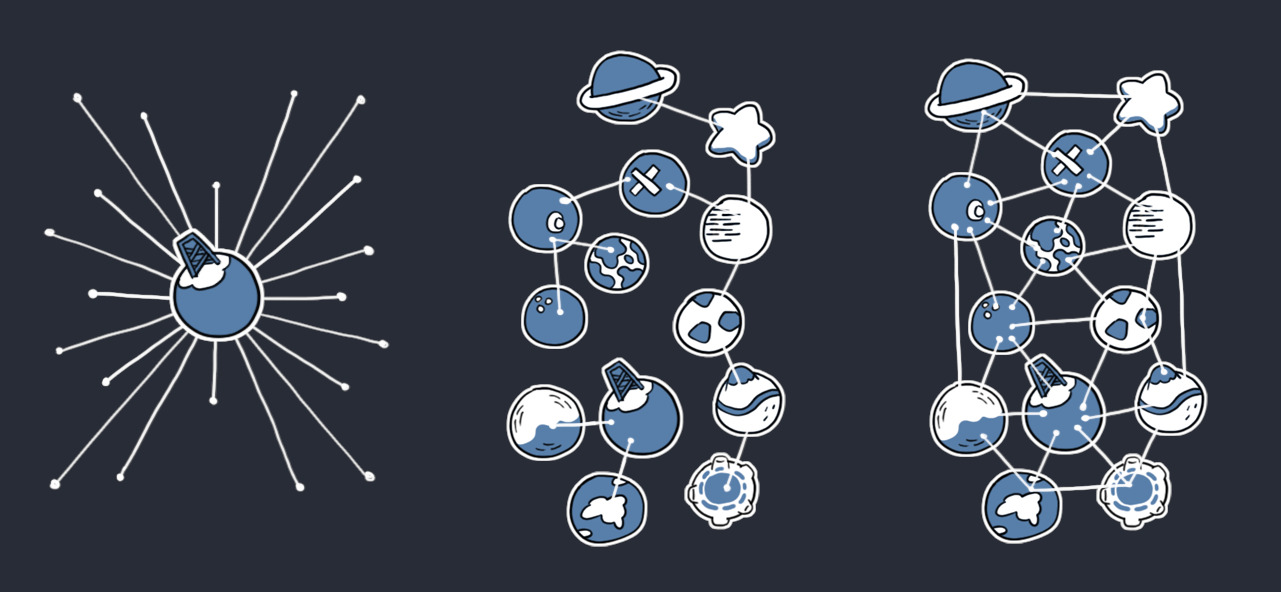
\includegraphics[width=\textwidth]{../material/network_models.jpg}
    \caption{From left to right: Centralized networks funnel all connections through a single controlling hub; Federated networks organize nodes into semi-autonomous interconnected clusters; Distributed networks connect all nodes with multiple pathways, maximizing resilience through decentralization. \cite{mastodon:docs}}
    \label{fig:network-models}
\end{figure}

To study the behavior of online communities on Mastodon, we analyze a dataset containing around 1.8 billion public Mastodon posts, called toots, collected from 1000 instances over the whole year 2024. The dataset includes metadata and the posted content, enabling an analysis of toxicity trends across instances and the interactions between them. However, given the scale of the dataset, traditional data processing methods are insufficient. To address this challenge, we build a distributed data processing pipeline using the Ray framework \cite{moritz:2018}. Ray provides a scalable and efficient platform for handling large-scale data, enabling us to perform tasks such as data deduplication, language detection, and toxicity prediction in a distributed manner.

By building this pipeline, we aim to provide a scalable and reproducible framework for analyzing toxicity in large-scale social media datasets. The study not only contributes to understanding toxicity in federated social networks like Mastodon but also demonstrates the practical application of distributed computing frameworks like Ray for social media research. The pipeline's modular design allows for future extensions, such as incorporating additional toxicity models or adapting the workflow to other social media platforms.

\enlargethispage{\baselineskip}
\chapter{Related Work}

Research on online toxicity has primarily focused on centralized social media platforms like Twitter and Facebook \cite{fan:2022,nicholson:2023}. These studies have examined various aspects of toxic behavior, including its diffusion patterns, impact on communities, and moderation strategies. However, decentralized online social networks (DOSNs) like Mastodon present unique challenges and opportunities for studying toxicity due to their federated architecture and distributed moderation systems \cite{bono:2024}. This chapter reviews relevant literature on Mastodon communities, decentralized moderation, and large-scale toxicity analysis to situate our research within the existing work.

\paragraph{Behaviour of Mastodon Communities}
Mastodon has emerged as a prominent DOSN, offering an alternative to centralized platforms by enabling users to join independent instances that form a federated network \cite{zulli:2020}. Unlike traditional social media, Mastodon's architecture allows for diverse communities with distinct norms and moderation practices \cite{la_cava:2021}. Instances work independently but connect through ActivityPub, forming a network where content flows between servers \cite{mastodon:docs}. This setup enables researchers to study how communities form and users behave differently than on centralized platforms like Twitter, especially looking at how groups separate or interact across instances \cite{zignani:2018}.

The topology of Mastodon communities exhibits unique characteristics. \citet{zulli:2020} found that Mastodon instances often form around specific interests, identities, or ideologies, leading to more homogeneous communities. This clustering behavior influences information consumption patterns and user relationships, with instances developing distinct footprints based on their thematic focus \cite{la_cava:2021}. Such organizational differences suggest that toxicity patterns in Mastodon may follow different dynamics than those observed in centralized platforms.

\paragraph{Decentralized Moderation Challenges}
The federated nature of Mastodon introduces novel challenges for content moderation, as each instance maintains its own policies and enforcement mechanisms. \citet{bono:2024} found that instance administrators primarily rely on blocklisting to moderate content, preventing users from interacting with servers hosting harmful material. This decentralized approach allows for customized moderation but creates inconsistencies across the network, as blocklisting decisions vary significantly between instances \cite{nicholson:2023}. The study found that blocklists mainly ban instances containing spam, hate speech, or adult content. Many administrators use these shared blocklists without carefully checking them first \cite{bono:2024}.

\citet{nicholson:2023} examined Mastodon's rules and discovered they focus more on preventing harassment and hate speech than similar Reddit communities. Their research showed that Mastodon's decentralized approach creates different types of rules across instances. Some rules specifically target e.g.,discrimination, while others use general community guidelines. Because each instance has its own moderation approach, studying toxicity becomes more challenging, as what users see and experience varies significantly depending on which instance they join.

\paragraph{Large-Scale Toxicity Analysis}
Existing approaches to toxicity analysis have typically focused on specific events or short timeframes on centralized platforms. For example \citet{fan:2022} developed a comprehensive workflow for analyzing toxicity during health crises, combining topic modeling and network analysis to understand toxic discourse patterns. Their approach, which processed over 1.6 million tweets during the 2022 Mpox outbreak, revealed how toxicity spreads differently through mentions versus retweets and identified influential users in toxic discourse networks \cite{fan:2022}.

The scale and distributed nature of Mastodon data require specialized processing pipelines. Existing research has highlighted the need for efficient deduplication methods when analyzing federated content, as posts often propagate across multiple instances \cite{bono:2024}.

\paragraph{Research Gap and Contribution}
Prior work has established foundational knowledge about Mastodon's structure \cite{zulli:2020,la_cava:2021}, moderation practices \cite{bono:2024,nicholson:2023}, and toxicity analysis methods \cite{fan:2022}. However, no study has systematically examined toxicity patterns across the entire Mastodon network while accounting for its federated architecture. Our research addresses this gap by conducting the first large-scale toxicity analysis of Mastodon, incorporating instance-specific moderation contexts and employing distributed computing techniques to handle the platform's scale. By analyzing a 10\% subsample out of 1.8 billion toots across 1,000 instances crawled over the whole year 2024, we provide insights into how toxicity manifests in DOSNs and how different moderation approaches affect its prevalence.
\chapter{Mastodon Dataset} \label{mastodon-dataset}
The dataset used in this study consists of public Mastodon posts (called ``toots'') collected from a federated network of instances. The data was gathered using a distributed crawler developed by \citet{ernst:2024}, which collects posts from Mastodon instances' public timelines via their REST API while respecting user privacy settings. The crawler stores the collected data in an Elasticsearch cluster with careful attention to ethical considerations, never publishing raw user data.

As reported by \citet{ernst:2024} in November~2024, the corpus contained 3.6~billion posts collected over 301~days from 1,081~instances. The complete dataset includes detailed metadata about each post and relationships between instances, with key fields described in Table~\ref{dataset-fields}. After deduplication, this resulted in 174~million unique posts, indicating a duplication rate of approximately 95\%\@, which reflects the federated nature of Mastodon where content is shared across instances. While the crawler has continued running since that report, our analysis focuses specifically on English-language toots from the complete year~2024, collected from 1,000~fully crawled instances.

\begin{table}[tb]
    \centering\small
    \renewcommand{\arraystretch}{1.3}
    \begin{tabularx}{\textwidth}{lX}
        \toprule
        \textbf{Field} & \textbf{Description} \\
        \midrule
        \texttt{id} & Unique identifier for each toot \\
        \texttt{content} & The post content in HTML format (converted to plain text for analysis) \\
        \texttt{crawled\_from\_instance} & The instance where the toot was observed \\
        \texttt{instance} & The home instance of the posting user \\
        \texttt{is\_local} & Boolean indicating whether the post originated on the crawled instance \\
        \texttt{created\_at} & Timestamp of post creation \\
        \texttt{sensitive} & Flag marking potentially sensitive content \\
        \texttt{spoiler\_text} & Content warnings or spoiler alerts \\
        \bottomrule
    \end{tabularx}
    \caption{Key fields available in the Mastodon dataset with their descriptions.}
    \label{dataset-fields}
\end{table}

The original corpus analysis revealed significant diversity in the data sources. While most posts originate from Mastodon instances, notable contributions come from other federated platforms like Misskey and RSS~Parrot. English (34.71\%) and Japanese (23.39\%) dominate the language distribution, with all other languages below 5\% each. Approximately 18\% of posts contain media attachments (mostly images), while 24\% include URL preview cards. Because our toxicity detection models just analyze text content, we removed those with media attachments. As well, we filtered out reblogs to reduce the dataset and focus on original posts. The final dataset contains around 1.8~billion toots. Becuase of the lack of time, we only analyze a 10\% subsample of the dataset in this study.
\chapter{Large-Scale Toxicity Analysis Pipeline} \label{large-scale-pipeline}
This chapter describes the technical workflow for processing and analyzing toxicity in social media posts, specifically focusing on English-language toots from Mastodon instances. The pipeline is built using the Ray framework \cite{moritz:2018}, which enables distributed computing for efficient large-scale data processing. The pipeline consists of several stages: data reading, deduplication, toxicity prediction, and merging. Each stage is designed to handle large datasets efficiently, leveraging parallel processing and optimized memory usage.

\paragraph{Prerequisites}
The Ray environment is configured with specific settings to ensure efficient processing of large datasets.
\todo[inline]{describe the parameters used in \textit{map\_batches} to get a good perforamce on our cluster}
To ensure robustness, the pipeline is configured to retry failed tasks up to 10 times, with retry exceptions enabled to handle transient errors gracefully.

These settings ensure that the pipeline can handle large datasets efficiently on our cluster while minimizing resource contention. The use of \textit{map\_batches} in the pandas format allows for seamless integration with data processing functions, enabling parallel execution of tasks.

\section{Reading and Processing Toots}\label{step:ingestion} 
The pipeline's first stage retrieves Mastodon data from Elasticsearch using the following filters:

\begin{enumerate}
    \item \textbf{Temporal scope}: Only toots posted during 2024
    \item \textbf{Instance selection}: From 1,000 fully crawled instances
    \item \textbf{Content filters}:
    \begin{itemize}
        \item Original toots only (excluding reblogs/boosts)
        \item Text-only content (removing toots with media attachments)
        \item English-language labeled content
    \end{itemize}
\end{enumerate}

We use the \textit{ray\_elasticsearch}\footnote{\url{https://github.com/janheinrichmerker/ray-elasticsearch}} library for efficient Elasticsearch queries. The retrieved data contains the fields described in Table~\ref{dataset-fields}, including toot identifiers, content, instance information, and metadata flags. To avoid overloading the Elasticsearch cluster, we read data directly into local storage using the Parquet\footnote{\url{https://github.com/apache/parquet-java}} file format for efficient storage.

For our toxicity analysis, we use a 10\% subsample of the dataset due to time constraints. To obtain the subsample we apply the \textit{sample} method from the pandas library before further processing.

The subsample data is processed to extract plaintext from the HTML content using the \textit{extract\_plain\_text} function from resiliparse \cite{bevendorff:2018}. This function extracts the main content of the toot, discarding any formatting or alternative texts. Empty or whitespace-only plaintexts are filtered out, and the original content column is dropped to reduce memory usage. Before writing to Parquet files, we calculate the MinHash for each toot's plaintext and write it into a new \textit{minhash} column. The MinHash provides an efficient way to estimate the Jaccard similarity between documents. The Jaccard similarity $J(A,B)$ between two sets $A$ and $B$ is defined as:

\begin{equation}
J(A,B) = \frac{|A \cap B|}{|A \cup B|}
\end{equation}

MinHash works by computing multiple hash values for each document's shingles (contiguous subsequences of words) and keeping only the minimum hash value for each permutation. The probability that the minimum hash values match for two toots equals their Jaccard similarity \cite{broder:2000}. Our implementation uses 64 permutations to balance storage requirements with similarity estimation accuracy. These MinHashes support deduplication and merging in subsequent pipeline stages.

\begin{figure}[tb]
    \centering
    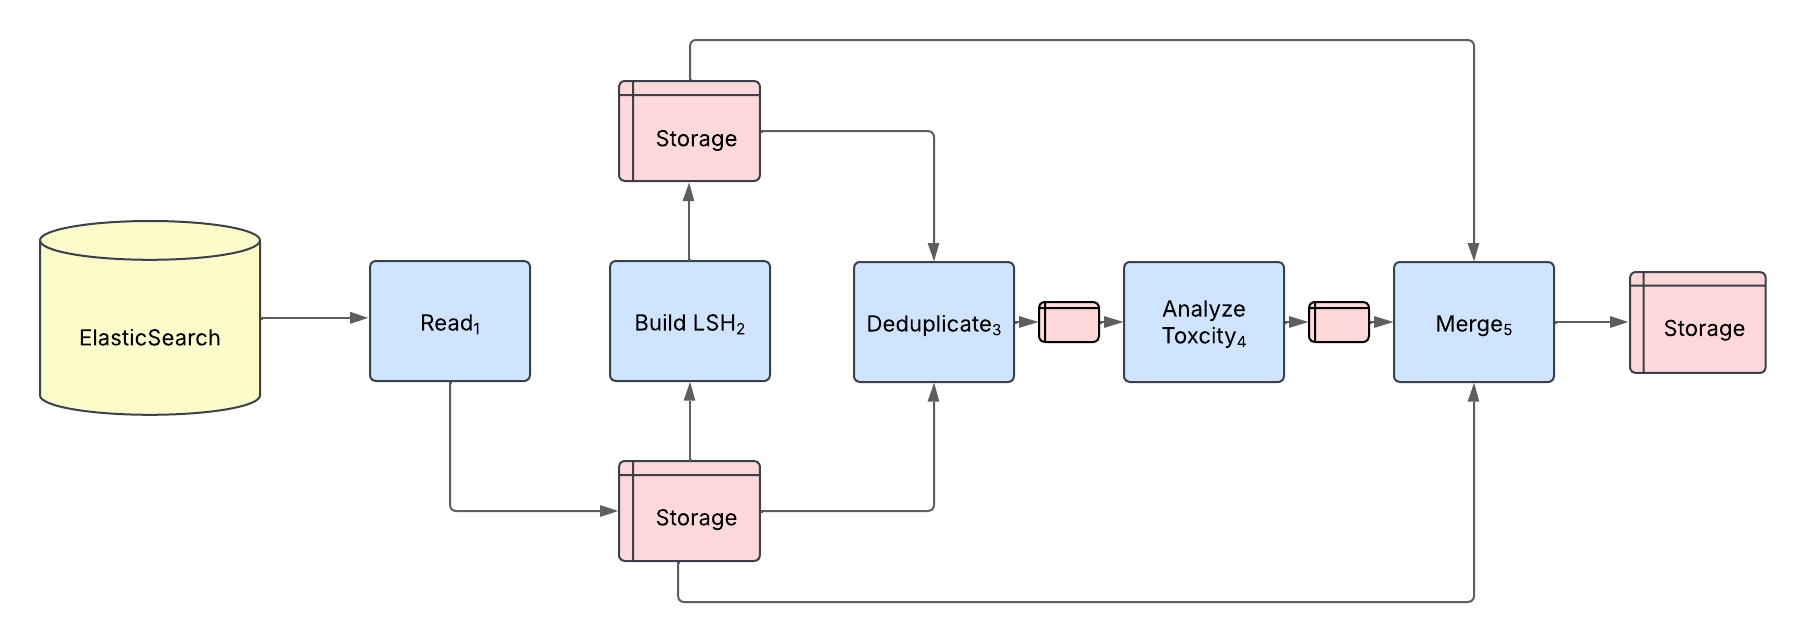
\includegraphics[width=\textwidth]{../material/pipeline.png}
    \caption{Data processing pipeline: 
    (\hyperref[step:ingestion]{1}) \textbf{Read \& Preprocess}: Reading data from the ElasticSearch database, extracting plaintext and calculating MinHash, then storing results; 
    (\hyperref[step:lsh]{2}) \textbf{Build LSH}: Building LSH index from processed data and storing it; 
    (\hyperref[step:dedup]{3}) \textbf{Deduplicate}: Near-duplicates are removed from processed data using the LSH index; 
    (\hyperref[step:toxicity]{4}) \textbf{Analyze Toxicity}: Performing toxicity analysis on deduplicated data; 
    (\hyperref[step:merge]{5}) \textbf{Merge}: Merging analyzed data with the original dataset using the LSH index. 
    Blue boxes represent processes, red indicates storage components, and yellow marks the external database.}
    \label{fig:pipeline}
\end{figure}

\section{LSH Index Construction and Toots Deduplication}\label{step:lsh_dedup} 
The deduplication stage employs Locality-Sensitive Hashing (LSH) techniques to efficiently identify and remove near-duplicate toots from the dataset. The idea of LSH is to group similar toots into buckets through a process called banding. This approach works by dividing each document's MinHash signature into $b$ bands of $r$ rows each. For a document with a MinHash signature of length $n$, we ensure $b \times r \le n$. Each band is then processed separately through a hash function, and toots sharing identical hash values in any band are considered potential duplicates. By setting the jaccard similarity threshold to 0.9, the optimizer finds values for $b$ and $r$ so that the probability of two toots sharing a band is very high when their Jaccard similarity is $\geq90\%$. The threshold is chosen to 0.9 because jaccard similarity is just indicating word similarity but not semantic similarity. Because we don't want to remove toots that are just similar in words but not in meaning, we choose a much higher threshold than the maybe more realistic threshold of 0.58 explored by \citet{wu:2020} for similarity in short texts.

\paragraph{LSH index construction}\label{step:lsh} The LSH index construction begins by reading the data from Parquet files generated in the previous processing stage. We just load two cloumns: the unique identifier (\textit{\_id}), and the precomputed MinHash values. These MinHash signatures are inserted into an LSH instance configured with our 0.9 similarity threshold. To optimize performance, we build multiple LSH instances in parallel using \textit{map\_batches}, then merge them into a single unified index. This merging is facilitated by Ray Actors, which provide stateful workers that maintain their internal state between operations. Unlike stateless functions, these actors allow us to incrementally build and combine LSH indexes while keeping memory usage manageable. The final consolidated LSH index is persisted as a pickle file for subsequent deduplication steps.

\paragraph{Deduplication}\label{step:dedup} During the deduplication phase, we now read three columns from the source Parquet files: the unique identifier (\textit{\_id}), the plaintext and the precomputed MinHash values. Additionally we load the prebuilt LSH index. For each toot we query the LSH index by inserting one minhash and receving all \textit{\_id}s in the same bucket. Those \textit{\_id}s belong to toots with Jaccard similarity of at least 90\%. Within each group of near-duplicates, we retain only the toot with the smallest \textit{\_id} value, ensuring deterministic selection while removing duplicates. This approach guarantees that only one representative instance of each near-duplicate group remains in the final dataset. The deduplicated results are then written back to Parquet files for further analysis and processing.

\section{Toxicity Analysis using Transformer-based Models}\label{step:toxicity}
After deduplication, the next stage involves predicting the toxicity of the deduplicated toots. This is done using pre-trained models designed to detect toxic content in text. The toxicity prediction is done in two main steps: language detection, and predicting toxicity labels.

\paragraph{Transformer-based Models}
Modern toxicity detection systems rely on Transformer-based language models, which have revolutionized natural language processing through their ability to learn contextualized word representations. The Transformer architecture, introduced by \citet{vaswani:2017}, works differently than older systems: instead of processing words one after another, it looks at all words in a sentence simultaneously. This allows it to better understand how distant words relate to each other, which is very important for detecting toxicity where harmful meaning often appear from combinations of words across a message."

Building on this foundation, \citet{devlin:2019} proposed Bidirectional Encoder Representations from Transformers (BERT), which introduced two key innovations. First, BERT trains by hiding random words in a sentence (like filling in blanks) and predicting them using both left and right context. This differs from older models that could only use previous words. Second, BERT learns whether two sentences logically follow each other, helping it understand conversation flow. These innovations enable BERT to create deep bidirectional representations that can be fine-tuned for downstream tasks with minimal architectural changes. The three toxicity detection models used in this study all use Transformer architectures.

% - just trained english text
% - trained on the "Jigsaw Toxic Comment Classification Challenge" dataset
% - dataset is build from wikipedia comments
% - labels like in table 5.1 but without sexual explicit
% - transformer-based model bert-base-uncased
% - fine-tuned on the Jigsaw... dataset
% - during prediction, input text is tokenized and passed through the transformer model
% - output is a probability score for the labels

\textbf{Detoxify Original}\footnote{\url{https://huggingface.co/unitary/toxic-bert}} is trained on English text using the "Jigsaw Toxic Comment Classification Challenge" dataset, which comprises Wikipedia comments. The model predicts probability scores for toxicity labels, which include categories similar to those listed in Table~\ref{toxicity-categories}, but without the sexually explicit label. The model is based on the BERT-base-uncased transformer architecture and fine-tuned on the Jigsaw dataset. During prediction, the input text is tokenized and processed through the transformer model to generate the output scores \cite{detoxify:medium}.

% - just trained english text
% - trained on the "Jigsaw Unintended Bias in Toxicity Classification" dataset
% - dataset is build from "Civil Comments" comments
% - labels like in table 5.1
% - for the training there are additional labels for identities, to reduce bias between different groups
% - transformer-based model roberta-base
% - fine-tuned on the Jigsaw... dataset
% - during prediction, input text is tokenized and passed through the transformer model
% - output is a probability score for the labels

\textbf{Detoxify Unbiased}\footnote{\url{https://huggingface.co/unitary/unbiased-toxic-roberta}} also focuses on English text but is trained on the "Jigsaw Unintended Bias in Toxicity Classification" dataset. This dataset consists of comments from "Civil Comments" platform and includes additional labels for identities to reduce bias across different demographic groups. The labels align with those in Table~\ref{toxicity-categories}. The model employs the RoBERTa-base transformer architecture and is fine-tuned on the Jigsaw dataset. Like Detoxify Original, it tokenizes input text and processes it through the transformer model to produce probability scores for the labels \cite{detoxify:medium}.

% - trained with multiple languages
% - For languages where less forum data is available, they use machine translation to translate labeled English-language comments into the target language.
% - training dataset is build from  variety of sources, including comments from online forums such as Wikipedia and The New York Times
% - Each comment is tagged by 3-10 crowdsourced raters
% - labels like in table 5.1 
% - start by training multilingual BERT-based models on data from online forums
% - distill these models into single-language Convolutional Neural Networks (CNNs) for each supported language
% - output is a probability score for the labels

\textbf{Perspective API} supports multiple languages and addresses the challenge of limited forum data for some languages by using machine translation. Labeled English-language comments are translated into the target language to supplement training data. The training dataset is sourced from diverse platforms, including Wikipedia and The New York Times, with each comment annotated by 3--10 crowdsourced raters. The labels match those in Table~\ref{toxicity-categories}. The training process begins with multilingual BERT-based models trained on the dataset, which are then distilled into single-language Convolutional Neural Networks (CNNs) for each supported language. As well as the two Detoxify models, the Perspective API outputs probability scores for the toxicity labels \cite{lees:2022}.

\paragraph{Language Detection using FastText}
To ensure only English texts are processed, a language detection step is performed. While the initial query filters for English-labeled toots, many are mislabeled. This additional filtering is critical because the toxicity prediction models from unitary cannot handle other languages.
For language detection, the deduplicated data is read from the Parquet files, and each task loads the FastText\footnote{\url{https://huggingface.co/facebook/fasttext-language-identification}} model. The model predicts the language of each toot’s plaintext, retaining only those labeled as English for further analysis.
FastText is ideal for this task due to its use of subword information (character n-grams), which enables robust handling of informal language, misspellings, and slang common in social media texts. Its efficiency and accuracy in language detection ensure reliable filtering, even for short or noisy inputs \cite{joulin:2016}.

\paragraph{Toxicity Prediction}
For toxicity classification, the selected toxicity model is loaded. For Detoxify models, this involves loading a transformer pipeline with truncation and padding enabled. For the Perspective API, the Google API client is used to make requests. We had to add a delay to respect the API's rate limit of 50 requests per second. The toxicity labels are predicted for each toot, and the results are appended to the dataset. The final dataset, including toxicity labels, is written back to Parquet files.

\section{MinHash-based Similarity Merging}\label{step:merge}
The final stage of the pipeline merges the toxicity labels back into the original dataset, ensuring the toxicity information is available for all toots—not just the deduplicated subset. The complete dataset is read from the Parquet files generated during the data reading stage. For each toot’s plaintext, the MinHash is computed, and the LSH index is queried to find similar toots. The smallest \textit{\_id} in the query results matches an \textit{\_id} in the deduplicated dataset. The toxicity labels corresponding to this \textit{\_id} are then concatenated with the queried toot. Finally, the toot, now containing all relevant information, is added to the final dataset, which is written back to Parquet files for further analysis.
\chapter{Choosing Transformer-based Toxicity Analyzer} \label{choosing-toxicity-analyzer}
To predict the toxicity of toots, we evaluated three models: Detoxify (Original), Detoxify (Unbiased) from Unitary, and Perspective API. These models predict probabilities for six to seven toxicity categories.

\section{Mastodon Posts Annotation} \label{annotation}
All models were evaluated on a subset of the dataset. The selected timeframe was the evening of the 2024 Paris Olympic Games' opening ceremony, chosen due to the expectation of heightened online discussions and increased toxic content. The dataset covers the period from 20:00 to 23:00 on July~26, 2024, comprising 1,179,897 toots. This context switch may impact model performance but also demonstrates robustness in a new context.

After predictions were completed, a sample was drawn for each model, selecting 25 toots per toxicity category with a predicted probability greater than 0.5. The selected toots were concatenated, and duplicates were removed, resulting in a final annotation dataset of 253 toots.

Two researchers conducted the annotation process using Label Studio. The toots were labeled according to the categories in Table~\ref{toxicity-categories}. Hate speech annotation is highly subjective and influenced by annotator biases, affecting consistency and reliability. To ensure reliability, inter-annotator agreement was measured using Cohen's Kappa. The results showed perfect agreement (Cohen's Kappa = 1.0) for the categories toxic, severe toxic, threat, insult, and identity attack. Near-perfect agreement was achieved for obscene (Cohen's Kappa = 0.9907) and sexually explicit (Cohen's Kappa = 0.9735), indicating high consistency between annotators.

\begin{table}[tb]
    \centering\small
    \renewcommand{\arraystretch}{1.3}
    \begin{tabularx}{\textwidth}{lX}
        \toprule
        \textbf{Category} & \textbf{Description} \\
        \midrule
        TOXIC & A rude, disrespectful, or unreasonable comment that is likely to make someone leave a discussion. \\
        SEVERE TOXIC & A very hateful, aggressive, or disrespectful comment that is highly likely to push someone away. \\
        IDENTITY ATTACK & Negative or hateful comments targeting someone because of their identity. \\
        INSULT & Insulting, inflammatory, or negative comments towards a person or group. \\
        OBSCENE & Swear words, curse words, or other obscene or profane language. \\
        THREAT & Describes an intention to inflict pain, injury, or violence against an individual or group. \\
        SEXUALLY EXPLICIT & Genital nudity or descriptions of simulated or actual sexual acts. \\
        \bottomrule
    \end{tabularx}
    \caption{Toxicity Categories and Their Descriptions}
    \label{toxicity-categories}
\end{table}

\section{Transformer-based Model Evaluation} \label{evaluation}
The evaluation focused on the probability distributions of toxicity categories and the F1 scores across the three models: Perspective API, Detoxify (Original), and Detoxify (Unbiased). The F1 score, calculated as:

\[
F1 = 2 \times \frac{\text{precision} \times \text{recall}}{\text{precision} + \text{recall}},
\]

was used to measure prediction performance, as it balances precision and recall.

A fixed threshold of 0.5 was used to compare F1 scores. The Perspective API model generally outperformed the Detoxify models in F1 scores for most categories (see Table~\ref{table-performance-metrics}). However, the probability distributions (Figure~\ref{probability-distribution}) revealed behavioral differences. The Perspective API model exhibited a widely spread distribution, suggesting cautious predictions, while the Detoxify models showed concentrated distributions, indicating higher confidence.

\begin{figure}[tb]
    \centering
    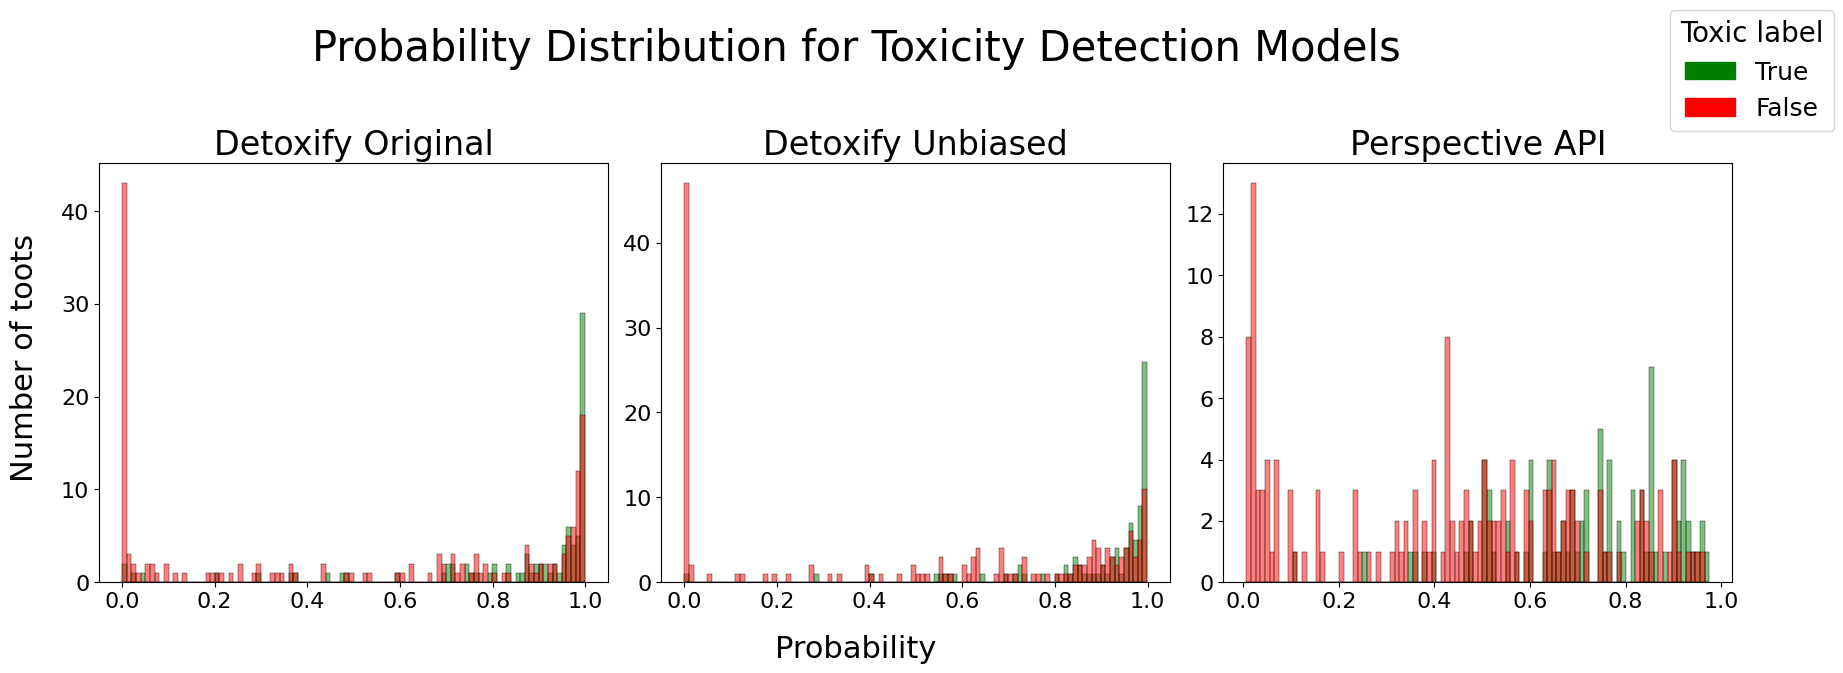
\includegraphics[width=\textwidth]{../material/probability_distribution.png}
    \caption{Probability Distribution of Toxicity category across the three models}
    \label{probability-distribution}
\end{figure}

The Perspective API model's limited accessibility, due to low request rates and lack of open access, posed practical constraints for large-scale analysis. In contrast, the open-source Detoxify models offered unrestricted usage, making them more suitable for extensive studies. Since the research goal is to analyze broader toxicity trends rather than individual toots, the Detoxify models were deemed more appropriate. A confident model like Detoxify is better for tracking trends over time.

Between the two Detoxify models, the unbiased version was selected for further analysis due to its superior performance (Table~\ref{table-performance-metrics}) and inclusion of the "sexual explicit" category, absent in the original model. However, the "severe toxic" label in the unbiased model performed poorly, likely due to limited supporting toots (only 10 in the dataset). Findings for this category should be interpreted cautiously. Despite this, the Detoxify unbiased model was chosen for analyzing Mastodon toxicity trends, balancing performance, accessibility, and practicality.

\begin{table}[p]
    \centering\small
    \caption{Performance metrics across toxicity categories with highest F1 scores highlighted.}
    \label{table-performance-metrics}
    \begin{tabular}{@{}lrrrr@{}}
      \toprule
      \textbf{Model} & \textbf{F1} & \textbf{Precision} & \textbf{Recall} & \textbf{Support} \\
      \midrule
      \multicolumn{5}{c}{\bfseries toxic} \\
      Detoxify Original      & 0.622 & 0.482 & 0.878 & 90 \\
      Detoxify Unbiased      & 0.635 & 0.473 & 0.967 & 90 \\
      Perspective API        & \textbf{0.664} & 0.526 & 0.900 & 90 \\
      \addlinespace[0.5em]
      
      \multicolumn{5}{c}{\bfseries severe toxic} \\
      Detoxify Original      & 0.148 & 0.118 & 0.200 & 10 \\
      Detoxify Unbiased      & 0.000 & 0.000 & 0.000 & 10 \\
      Perspective API        & \textbf{0.222} & 0.176 & 0.300 & 10 \\
      \addlinespace[0.5em]
      
      \multicolumn{5}{c}{\bfseries obscene} \\
      Detoxify Original      & \textbf{0.741} & 0.613 & 0.936 & 78 \\
      Detoxify Unbiased      & 0.739 & 0.642 & 0.872 & 78 \\
      Perspective API        & 0.738 & 0.615 & 0.923 & 78 \\
      \addlinespace[0.5em]
      
      \multicolumn{5}{c}{\bfseries threat} \\
      Detoxify Original      & 0.462 & 0.429 & 0.500 & 18 \\
      Detoxify Unbiased      & 0.520 & 0.406 & 0.722 & 18 \\
      Perspective API        & \textbf{0.596} & 0.483 & 0.778 & 18 \\
      \addlinespace[0.5em]
      
      \multicolumn{5}{c}{\bfseries insult} \\
      Detoxify Original      & 0.377 & 0.312 & 0.476 & 42 \\
      Detoxify Unbiased      & \textbf{0.500} & 0.378 & 0.738 & 42 \\
      Perspective API        & 0.487 & 0.384 & 0.667 & 42 \\
      \addlinespace[0.5em]
      
      \multicolumn{5}{c}{\bfseries identity attack} \\
      Detoxify Original      & 0.440 & 0.314 & 0.733 & 15 \\
      Detoxify Unbiased      & \textbf{0.545} & 0.414 & 0.800 & 15 \\
      Perspective API        & 0.456 & 0.310 & 0.867 & 15 \\
      \addlinespace[0.5em]
      
      \multicolumn{5}{c}{\bfseries sexually explicit} \\
      Detoxify Original      & 0.000 & 0.000 & 0.000 & 21 \\
      Detoxify Unbiased      & 0.392 & 0.333 & 0.476 & 21 \\
      Perspective API        & \textbf{0.576} & 0.447 & 0.810 & 21 \\
      \bottomrule
    \end{tabular}
  \end{table}
\chapter{Analysis of Results} \label{results}

\chapter{Discussion} \label{discussion}


% Bibliography
\bibliographystyle{plainnat} % requires package natbib. An alternative is apalike
\bibliography{literature}    % load file literature.bib

\end{document}

